\setcounter{exo}{0}

\ifprof
\else
Soit le train d'engrenages suivant. 
\begin{center}
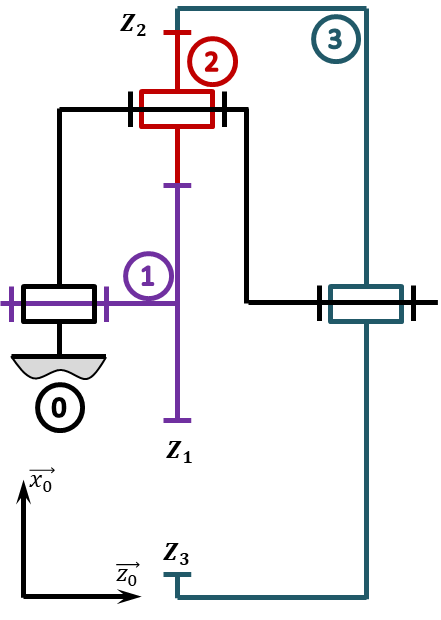
\includegraphics[width=.6\linewidth]{TrainSimple_01}
\end{center}
\fi

\subparagraph{}
\textit{Déterminer $\dfrac{\omega_{3/0}}{\omega_{1/0}}$ en fonction du nombre de dents des roues dentées.}
\ifprof
\begin{corrige}
On a $\dfrac{\omega_{3/0}}{\omega_{1/0}}=-\dfrac{Z_1}{Z_3}$.
\end{corrige}
\else
\fi

\subparagraph{}
\textit{Donner une relation géométrique entre $Z_1$, $Z_2$ et $Z_3$ permettant de garantir le fonctionnement du train d'engrenages. }
\ifprof
\begin{corrige}
On a $Z_3 = 2Z_2 + Z_1$.
\end{corrige}
\else
\fi



\ifprof
\else
Soit le train d'engrenages suivant. 
\begin{center}
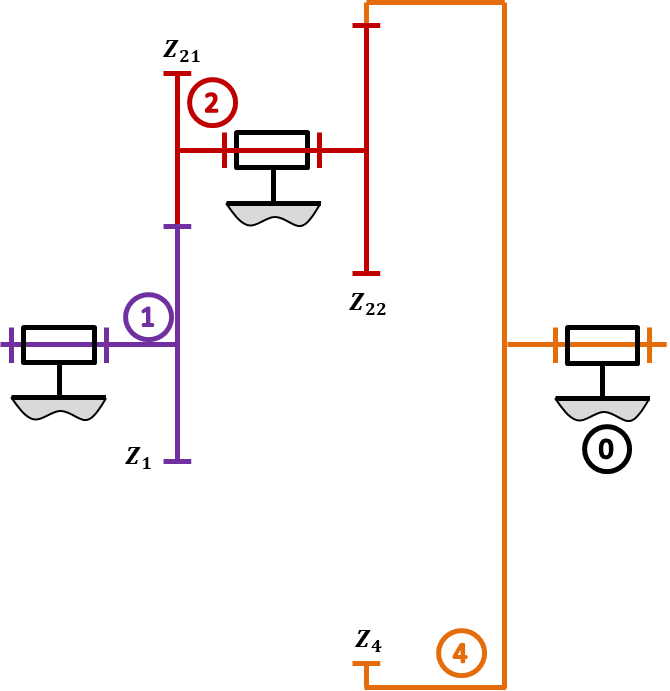
\includegraphics[width=.7\linewidth]{TrainSimple_02}
\end{center}
\fi

\subparagraph{}
\textit{Déterminer $\dfrac{\omega_{4/0}}{\omega_{1/0}}$ en fonction du nombre de dents des roues dentées.}
\ifprof
\begin{corrige}
On a $\dfrac{\omega_{4/0}}{\omega_{1/0}}=-\dfrac{Z_1Z_{22}}{Z_4Z_{21}}$.
\end{corrige}
\else
\fi

\subparagraph{}
\textit{Donner une relation géométrique entre $Z_1$, $Z_{21}$, $Z_{22}$ et $Z_4$ permettant de garantir le fonctionnement du train d'engrenages. }
\ifprof
\begin{corrige}
On a $Z_1+Z_{21}+Z_{22}= Z_4$.
\end{corrige}
\else
\fi



\ifprof
\else
Soit le train d'engrenages suivant. 
\begin{center}
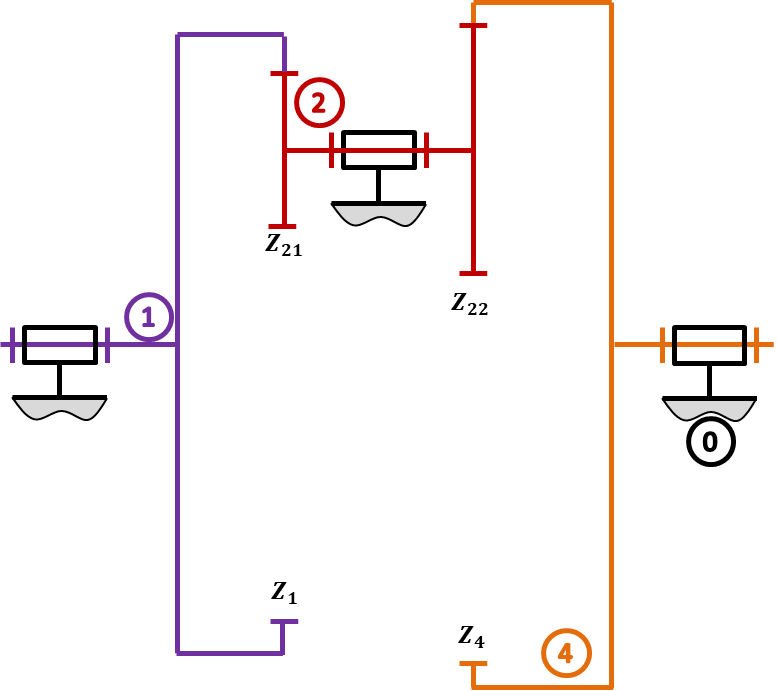
\includegraphics[width=.7\linewidth]{TrainSimple_03}
\end{center}
\fi


\subparagraph{}
\textit{Déterminer $\dfrac{\omega_{4/0}}{\omega_{1/0}}$ en fonction du nombre de dents des roues dentées.}
\ifprof
\begin{corrige}
On a $\dfrac{\omega_{4/0}}{\omega_{1/0}}=\dfrac{Z_1Z_{22}}{Z_4Z_{21}}$.
\end{corrige}
\else
\fi


\ifprof
\else
Soit le train d'engrenages suivant. 
\begin{center}
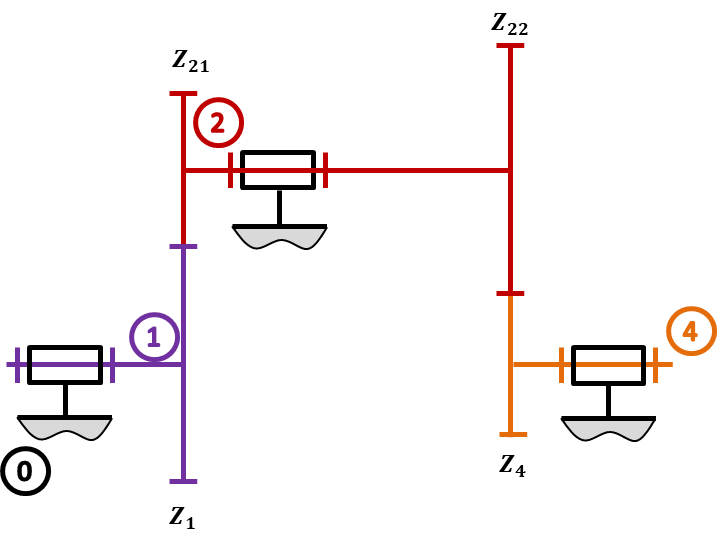
\includegraphics[width=.7\linewidth]{TrainSimple_04}
\end{center}
\fi


\subparagraph{}
\textit{Déterminer $\dfrac{\omega_{4/0}}{\omega_{1/0}}$ en fonction du nombre de dents des roues dentées.}
\ifprof
\begin{corrige}
On a $\dfrac{\omega_{4/0}}{\omega_{1/0}}=\dfrac{Z_1Z_{22}}{Z_4Z_{21}}$.
\end{corrige}
\else
\fi